% Hlavicka pro protokoly z fyzikalniho praktika.
% Verze pro: LaTeX
% Verze hlavicky: 22. 2. 2007
% Autor: Ustav fyziky kondenzovanych latek
% Ke stazeni: www.physics.muni.cz/ufkl/Vyuka/
% Licence: volne k pouziti, nejlepe k vcasnemu odevzdani protokolu z Vaseho mereni.

\documentclass[a4paper,11pt]{article}

% Kodovani (cestiny) v dokumentu: cp1250
% \usepackage[cp1250]{inputenc}	% Omezena stredoevropska kodova stranka, pouze MSW.
\usepackage[utf8]{inputenc}	% Doporucujeme pouzivat UTF-8 (unicode).
\usepackage{subfig}
\usepackage{float}

\usepackage{xparse}

\NewDocumentCommand{\codeword}{v}{%
\texttt{\textcolor{codepurple}{#1}}%
}

%%% Nemente:
\usepackage[margin=2cm]{geometry}
\newtoks\jmenopraktika \newtoks\jmeno \newtoks\datum
\newtoks\obor \newtoks\skupina \newtoks\rocnik \newtoks\semestr
\newtoks\cisloulohy \newtoks\jmenoulohy
\newtoks\tlak \newtoks\teplota \newtoks\vlhkost
%%% Nemente - konec.


%%%%%%%%%%% Doplnte pozadovane polozky:

\jmenopraktika={Fyzikální praktikum 1}  % nahradte jmenem vaseho predmetu
\jmeno={Milan Suk}            % nahradte jmenem mericiho
\datum={16. dubna 2018}        % nahradte datem mereni ulohy
\obor={F}                     % nahradte zkratkou vami studovaneho oboru
\skupina={PO 8:00}            % nahradte dobou vyuky vasi seminarni skupiny
\rocnik={I}                  % nahradte rocnikem, ve kterem studujete
\semestr={II}                 % nahradte semestrem, ve kterem studujete

\cisloulohy={9}               % nahradte cislem merene ulohy
\jmenoulohy={Měření elektrického napětí a proudu} % nahradte jmenem merene ulohy

\tlak={97,9}                   % nahradte tlakem pri mereni (v hPa)
\teplota={21,4}               % nahradte teplotou pri mereni (ve stupnich Celsia)
\vlhkost={40}               % nahradte vlhkosti vzduchu pri mereni (v %)

%%%%%%%%%%% Konec pozadovanych polozek.


%%%%%%%%%%% Uzitecne balicky:
\usepackage[czech]{babel}
\usepackage{graphicx}
\usepackage{amsmath}
\usepackage{xspace}
\usepackage{url}
\usepackage{indentfirst}
\usepackage{listings}
\usepackage{color}


\definecolor{codegreen}{rgb}{0,0.6,0}
\definecolor{codegray}{rgb}{0.5,0.5,0.5}
\definecolor{codepurple}{rgb}{0.58,0,0.82}
\definecolor{backcolour}{rgb}{0.95,0.95,0.92}
 
\lstdefinestyle{mystyle}{
    backgroundcolor=\color{backcolour},   
    commentstyle=\color{codegreen},
    keywordstyle=\color{magenta},
    numberstyle=\tiny\color{codegray},
    stringstyle=\color{codepurple},
    basicstyle=\footnotesize,
    breakatwhitespace=false,         
    breaklines=true,                 
    captionpos=b,                    
    keepspaces=true,                 
    numbers=left,                    
    numbersep=5pt,                  
    showspaces=false,                
    showstringspaces=false,
    showtabs=false,                  
    tabsize=2
}
 
\lstset{style=mystyle}

%%%%%% Zamezeni parchantu:
\widowpenalty 10000 \clubpenalty 10000 \displaywidowpenalty 10000
%%%%%% Parametry pro moznost vsazeni vetsiho poctu obrazku na stranku
\setcounter{topnumber}{3}	  % max. pocet floatu nahore (specifikace t)
\setcounter{bottomnumber}{3}	  % max. pocet floatu dole (specifikace b)
\setcounter{totalnumber}{6}	  % max. pocet floatu na strance celkem
\renewcommand\topfraction{0.9}	  % max podil stranky pro floaty nahore
\renewcommand\bottomfraction{0.9} % max podil stranky pro floaty dole
\renewcommand\textfraction{0.1}	  % min podil stranky, ktery musi obsahovat text
\intextsep=8mm \textfloatsep=8mm  %\intextsep pro ulozeni [h] floatu a \textfloatsep pro [b] or [t]

% Tecky za cisly sekci:
\renewcommand{\thesection}{\arabic{section}.}
\renewcommand{\thesubsection}{\thesection\arabic{subsection}.}
% Jednopismenna mezera mezi cislem a nazvem kapitoly:
\makeatletter \def\@seccntformat#1{\csname the#1\endcsname\hspace{1ex}} \makeatother


%%%%%%%%%%%%%%%%%%%%%%%%%%%%%%%%%%%%%%%%%%%%%%%%%%%%%%%%%%%%%%%%%%%%%%%%%%%%%%%
%%%%%%%%%%%%%%%%%%%%%%%%%%%%%%%%%%%%%%%%%%%%%%%%%%%%%%%%%%%%%%%%%%%%%%%%%%%%%%%
% Zacatek dokumentu
%%%%%%%%%%%%%%%%%%%%%%%%%%%%%%%%%%%%%%%%%%%%%%%%%%%%%%%%%%%%%%%%%%%%%%%%%%%%%%%
%%%%%%%%%%%%%%%%%%%%%%%%%%%%%%%%%%%%%%%%%%%%%%%%%%%%%%%%%%%%%%%%%%%%%%%%%%%%%%%

\begin{document}

%%%%%%%%%%%%%%%%%%%%%%%%%%%%%%%%%%%%%%%%%%%%%%%%%%%%%%%%%%%%%%%%%%%%%%%%%%%%%%%
% Nemente:
%%%%%%%%%%%%%%%%%%%%%%%%%%%%%%%%%%%%%%%%%%%%%%%%%%%%%%%%%%%%%%%%%%%%%%%%%%%%%%%
\thispagestyle{empty}

{
\begin{center}
\sf 
{\Large Ústav fyzikální elektroniky Přírodovědecké fakulty Masarykovy univerzity} \\
\bigskip
{\huge \bfseries FYZIKÁLNÍ PRAKTIKUM} \\
\bigskip
{\Large \the\jmenopraktika}
\end{center}

\bigskip

\sf
\noindent
\setlength{\arrayrulewidth}{1pt}
\begin{tabular*}{\textwidth}{@{\extracolsep{\fill}} l l}
\large {\bfseries Zpracoval:}  \the\jmeno & \large  {\bfseries Naměřeno:} \the\datum\\[2mm]
\large  {\bfseries Obor:} \the\obor  \hspace{40mm}  {\bfseries Skupina:} \the\skupina %
&\large {\bfseries Testováno:}\\
\\
\hline
\end{tabular*}
}

\bigskip

{
\sf
\noindent \begin{tabular}{p{3cm} p{0.6\textwidth}}
\Large  Úloha č. {\bfseries \the\cisloulohy:} \par
&\Large \bfseries \the\jmenoulohy  \\[2mm]
\end{tabular}
}

%%%%%%%%%%%%%%%%%%%%%%%%%%%%%%%%%%%%%%%%%%%%%%%%%%%%%%%%%%%%%%%%%%%%%%%%%%%%%%%
% konec Nemente.
%%%%%%%%%%%%%%%%%%%%%%%%%%%%%%%%%%%%%%%%%%%%%%%%%%%%%%%%%%%%%%%%%%%%%%%%%%%%%%%

%%%%%%%%%%%%%%%%%%%%%%%%%%%%%%%%%%%%%%%%%%%%%%%%%%%%%%%%%%%%%%%%%%%%%%%%%%%%%%%
%%%%%%%%%%%%%%%%%%%%%%%%%%%%%%%%%%%%%%%%%%%%%%%%%%%%%%%%%%%%%%%%%%%%%%%%%%%%%%%
% Zacatek textu vlastniho protokolu
%%%%%%%%%%%%%%%%%%%%%%%%%%%%%%%%%%%%%%%%%%%%%%%%%%%%%%%%%%%%%%%%%%%%%%%%%%%%%%%
%%%%%%%%%%%%%%%%%%%%%%%%%%%%%%%%%%%%%%%%%%%%%%%%%%%%%%%%%%%%%%%%%%%%%%%%%%%%%%%


\section{Úvod}

    \paragraph{} V analogové části této plohy je cílem proměřit vnitřní odpor použitého
    ampérmetru a určit hodnoty pro bočník, resp. předřadník, aby s ním bylo možné měřit
    hodnoty pro nové zadané rozsahy. V digitální části se má zjistit rozsah užitých D/A
    převodníků, reálný rozsah napětí, kvantizační krok a rozlišovací schopnost. Nakonec 
    se má otestovat vliv vzorkovací frekvence na kvalitu záznamu analogového signálu.

\section{Postup měření}

    \paragraph{} (A) Nejdříve se měl vnitřní odpor ampérmetru určit z ohmova zákona. 
    Ampérmetr se připojil ke zdroji proudu a na svorkách ampérmetru se zároveň měřilo
    něptí digitálním volmetrem. (B) Při druhé metodě se volmetr nahradil odporovou dekádou.
    Nejdřív se změril proud $I$ na ampérmetru bez paralelně připojeného odporu. Poté 
    se hledala taková hodnota odporu, aby ampérmetr měřil polovinu původní hodnoty
    proudu $\frac{I}{2}$. Tím pádem nastavený odpor na dekádě odpovídá odporu v druhé
    větvi, tedy vnitřnímu odporu ampérmetru.

    \paragraph{} Velikost bočníku se hledala pro počáteční rozsah $I_{A} = 100 \mu A$
    a vnitřní odpor $R_{A}$.  Velikost bočníku se pro nový rozsah určí jako 
    $R_{B} = \frac{R_{A}}{n - 1}$. Odpor předřadníku se spočítá jako 
    $R_{P} = (\frac{U_{N}}{U_{V}} - 1) R_{V} = (\frac{U_{N}}{I_{A} R_{A}} - 1) R_{V}$. 

    \paragraph{} Napěťový rozsah převodníků určím jako rozdíl změřených hodnota napětí
    pro největší a nejmenší hodnota číselného rozsahu. Jelikož je závislost napětí na
    číselných hodnotách pokud možno lineární, lze jej určit jako napěťový rozsah 
    dělený číselným rozsahem. Kvantizační krok u dvanáctibitového A/D převodníku
    se má určit měřením napětí při zkratovaných svorkách. V naměřených datech stačí najít
    nejmenší změnu napětí, tato hodnota by měla odpovídat kvantizačnímu kroku.

\section{Výsledky}

    \subsection{Měření vnitřního odporu ampérmetru}

    \paragraph{} Při první metodě pro hodnotu $I = 100 \mu A$ naměřil voltmetr
    hodnotu $U = 180.04mV$. Vnitřní odpor zde vychází

    \begin{equation}
        R^{(1)} = 1800,4 \Omega
    \end{equation}

    \paragraph{} Pro metodu s bočníkem hodnota odporu vychází

    \begin{equation}
        R^{(2)} = 1790 \Omega
    \end{equation}

    \subsection{Měření odporu bočníku, resp. předřadníku}

         \begin{table}[h]
            \centering
                \begin{tabular}{ | l | l | l | }
                    \hline
                    $I_{N}$  & $n$ & $R_{B}$    \\ \hline
                    0,5 $mA$ & 5   & 450 $\Omega$ \\ \hline
                    1 $mA$   & 10  & 200 $\Omega$ \\ \hline
                    2 $mA$   & 20  & 95 $\Omega$  \\
                    \hline
                \end{tabular}
            \caption{Hodnoty odporů bočníků}
            \label{fig:method_b}
        \end{table}

         \begin{table}[h]
            \centering
                \begin{tabular}{ | l | l | l | }
                    \hline
                    $U_{N}$  & $\frac{U_{N}}{U_{V}} - 1$ & $R_{B}$        \\ \hline
                    5 $V$    & 27                        & 48 600 $\Omega$  \\ \hline
                    10 $V$   & 55                        & 99 000 $\Omega$  \\
                    \hline
                \end{tabular}
            \caption{Hodnoty odporů předřadníků}
            \label{fig:method_b}
        \end{table}

    \subsection{Digitální část}

         \begin{table}[h]
            \centering
                \begin{tabular}{ | l | l | l | l | l | l | }
                    \hline
                    typ převodníku  & číselný rozsah  & $U_0$          & $U_{max}$     & napěťový rozsah & kvantizační krok \\ \hline
                    8-bit D/A       & $2^{8} = 256$   & 0.001262 $V$   & 9.879249 $V$  & 9.877987 $V$    & 0.038586 $V$     \\ \hline
                    16-bit D/A      & $2^{16} = 65536$ & -10.675357 $V$ & 10.698079 $V$ & 21.373436 $V$   & 0.0003261 $V$    \\
                    \hline
                \end{tabular}
            \caption{Parametry převodníků}
            \label{fig:method_b}
        \end{table}

        \paragraph{} Pro nalezení číselné hodnoty odpovídající hledanému napětí stačí použít jednoduchý vztah.

        \begin{equation}
            k = \frac{c}{u} U
        \end{equation}

        kde jako $c$ jsem si označil číselný rozsah převodníku, $u$ napěťový rozsah a $U$ hledané napětí.
        Pro hledané napětí v zadání úlohy $3.2V$ vychází hledaná číselná hodnota pro 8-mibitový převodník
        mezi $82$ a $83$ (po změření $3.172783V$ a $3.209893V$), pro 16-tibitový mezi $42547$ a $42548$
        (po změření $3.199839V$ a $3.200263V$).

        \paragraph{} Kvantizační krok 12-tibitového převodníku určím následujícím Python scriptem.

\begin{lstlisting}[language=Python]
import numpy
import matplotlib.pyplot as plt

data = numpy.loadtxt("data.txt")
data_diffs = []

for i in range(len(data)):
    if i == 0:
        continue

    data_diffs.append(abs(data[i] - data[i - 1]))

data_sorted = numpy.unique(numpy.sort(data_diffs))

print(data_sorted[:20])

plt.plot(data_sorted, 'ro')
plt.show()\end{lstlisting} 

    \begin{figure}[h]
        \centering
        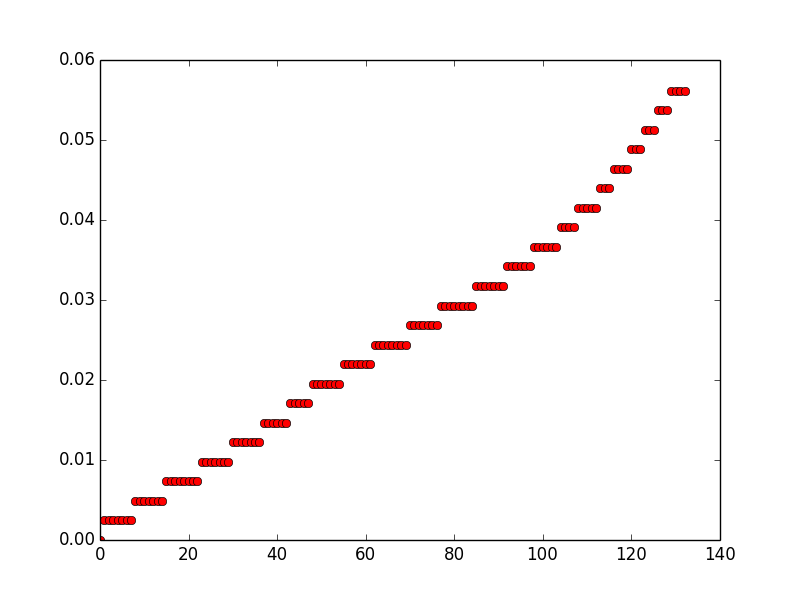
\includegraphics[width=0.6\linewidth]{diffs.png}
        \caption{Hodnoty rozdílů napětí}
    \end{figure}

    \paragraph{} Tedy kvantizační krok je $0.00244199V$.

    \paragraph{Vliv vzorkovací frekvence na kvalitu záznamu} V této úloze se testovalo, jaký vliv 
    má vzorkovací frekvence převodníku na kvalitu získaného záznamu analogového signálu. Největší
    problémem je, že při vykreslování záznamu předpokládáme, že získáné body v grafu jsou si blízké,
    takže je vykreslovací program generuje tím způsobem, že dva sousedící body spojí vhodnou funkcí
    - nejčastěji přímkou. Pro vyzkoušení jsem napsal jednoduchý program, který přesně tento proces
    simuluje. 

\begin{lstlisting}[language=Python][h]
import matplotlib.pyplot as plt
import numpy

freq = 3
f = 3

step = 1.0 / f
data = [numpy.sin(freq * x) for x in numpy.arange(0, 20, step)]
plt.plot(data)
plt.show()\end{lstlisting} 

    \paragraph{} Proměnná \codeword{freq} je frekvence generovaného signálu a \codeword{f} je
    snímkovací frekvence, ze které se generují body do definičního oboru $[0, 20]$.

    \begin{figure}[H]
        \centering
        \subfloat[1Hz]{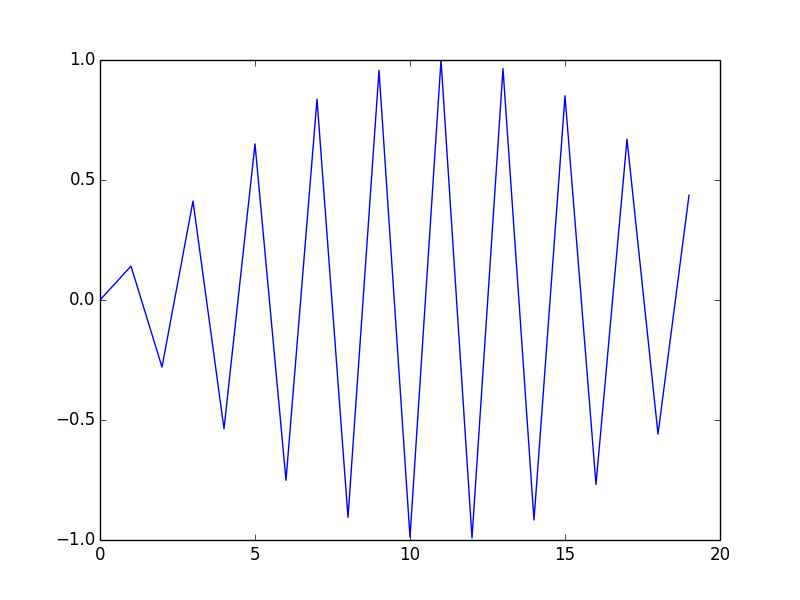
\includegraphics[width=0.2\textwidth]{freq_1.png}\label{fig:f2}}
        \subfloat[3Hz]{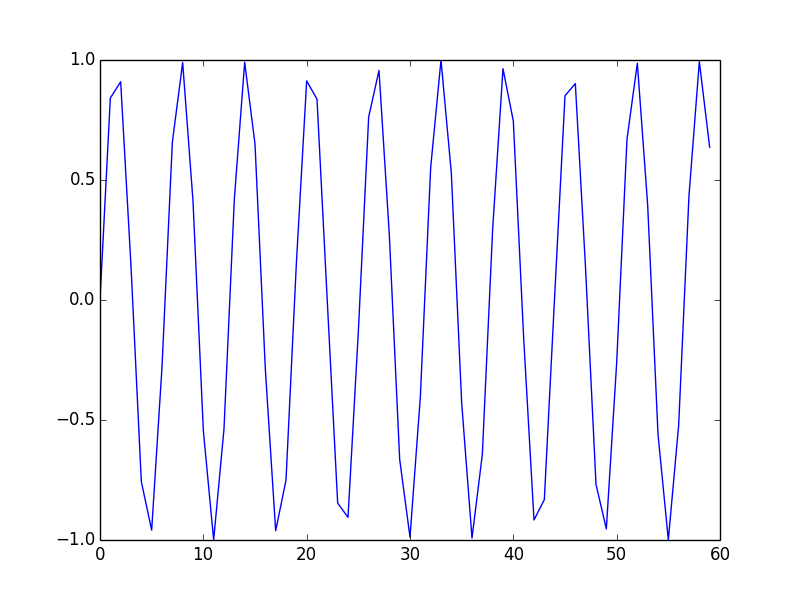
\includegraphics[width=0.2\textwidth]{freq_3.png}\label{fig:f1}}
        \subfloat[6Hz]{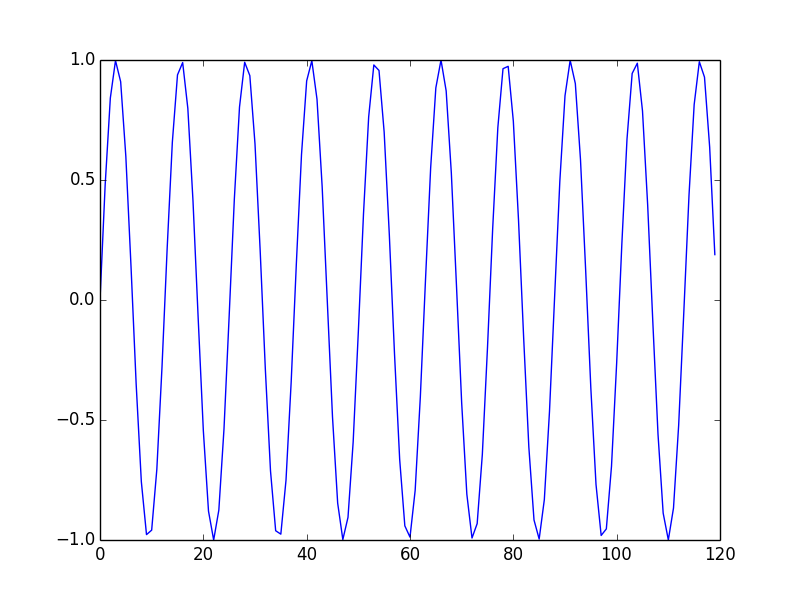
\includegraphics[width=0.2\textwidth]{freq_6.png}\label{fig:f2}}
        \caption{$sin(3x)$ snímaný různými frekvencemi}
    \end{figure}

    \paragraph{} Například při snímání frekvencí 1Hz se silně projevuje zmíněný efekt, že při špatně zvolených
    bodech snímání signálu a následným propojením bodů přímkou působý výsledný graf jako
    zcela jiná křivka a není vůbec zachycen charakter funkce $sin(3x)$. U frekvence 3Hz je již 
    alespoň zachycen tvar funkce a při dvojnásobné frekvenci už dostávám poměrně dobrý 
    záznam signálu.

\end{document}
